The main objective of Isar foundations is to turn existing formal logic concepts (natural deduction, minimal HOL, higher-order resolution and higher-order unification) into  a  viable  language  environment  for  natural  deduction  proof  texts (using concepts from high-level programming languages, leaving behing raw logic). The Isar/VM interpreter connects these two worlds.

Material for Isar: http://isabelle.in.tum.de/Isar/

\subsubsection{Outer\_Syntax and Toplevel}

Clicking at the Isar command we get this value:

\begin{lstlisting}
Outer_Syntax.command ("theory")  "begin theory"
	(Thy_Header.args >> (fn _ => Toplevel.init_theory 
		(fn () => error "Missing theory initialization")));
\end{lstlisting}

Here are two elements that define the parsing and collection of data useful for the internal proofs. 

The Outer\_Syntax structure defines the command function as:

\begin{lstlisting}
val command: command_keyword -> string ->
	(Toplevel.transition -> Toplevel.transition) parser -> unit
\end{lstlisting}

This can be understood as a meta-system transition with some functionality already suggested::

1. Produces as a side-effect a Toplevel.transition -> Toplevel.transition
2. Defines a new command relating its syntax and semantics to the given keyword. Notice that at this level a command is just a datatype with basic compiled information:

\begin{lstlisting}
datatype command = Command of
	{comment: string,
	command_parser: command_parser,
	pos: Position.T,
	id: serial};
\end{lstlisting}

3. Creates a basic theory and context, initializing the header of the theory and registers the Toplevel.transition -> Toplevel.transition to the Isar interpreter.
 
The Toplevel structure (see toplevel.ML) seems to take care of the registered data. It provides an internal state with the operations to pack and unpack theories and Proof.contexts on it. The extensibility of Isabelle as a system framework depends on a number of tables, into
which various concepts commands, ML-antiquotations, text-antiquotations, cartouches, can be entered via a late-binding on the fly.

This section is less well-understood than others. Rough reference is the Ecclectic Manual. However:

Can we debug the ML code as in a pure application?

Actually, it seems that file pure\_syn.ML is only charged of the basic syntax. 

\subsubsection{Isar/VM}

The command language has an interpreter (see proof.ML). Our primary concern here is to explain the virtual machine commands

\begin{figure}
	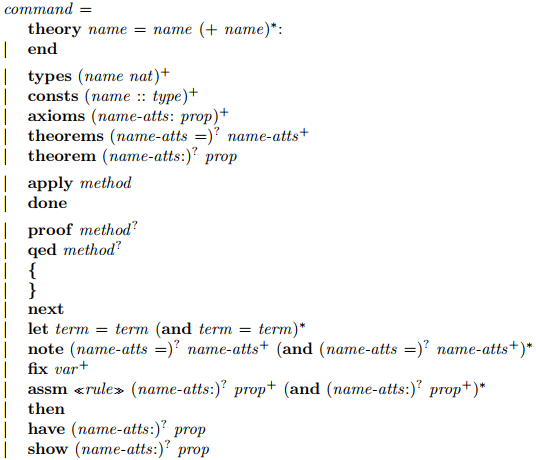
\includegraphics[scale=0.65]{img/commands.png}
\end{figure}










